\chapter{Experiments in investigating innovation ecosystems}
\label{ch:experiments}

In this chapter, we give an overview of the individual experiments on investigation innovation ecosystems with data-driven visual network analytics. In the context of this dissertation, the experiments serve first and foremost as means to develop the approach and methodology for investigating innovation ecosystems as networks, i.e. to distill design principles and process requirements in interaction with innovation ecosystem actors, stakeholder, decision-makers and investigators through the process of guided emergence \citep[cf.][]{Sein2011ActionResearch}. Moreover, the results and insights contribute to \ref{objective:empirical} of the dissertation.

The experiments are conducted on innovation ecosystems representing different levels of abstraction and complexity from Demola platform, a local ecosystem engager, to EIT ICT Labs (currently operating as EIT Digital), a large international ``open innovation organisation''\footnote{EIT Digital, \url{http://eit.europa.eu/eit-community/eit-digital}}. In all of the experiments, we take a data-driven approach to explore and describe the structure and in some cases structural dynamics of the innovation ecosystems under investigation.

The innovation ecosystems in which the experiments take place represent a broad range of abstraction and complexity. For specificity, we present the following categorization for the innovation ecosystems:

\begin{itemize} 
  \item Platform level: Demola
  \item Business domain level: Mobile Ecosystem 
  \item Program level: Tekes Young Innovative Companies\footnote{Tekes Young Innovative Company funding programme, \url{http://www.tekes.fi/en/funding/yic/}}
  \item National level: Finnish Innovation Ecosystem
  \item International level: EIT ICT Labs
\end{itemize}

Here, we will review the experiments from local to global. We want to note, however, that the order in which the experiments were conducted is different from the categorical order. Finnish Innovation Ecosystem was the first experiment. Second, the investigation of the mobile ecosystem was conducted. Third, we took a network approach to investigate the ecosystem emerging through Tekes Young Innovative Companies program. Fourth, means to use visualization to support orchestration of EIT ICT Labs were investigated. Fifth, we revisited the Finnish Innovation Ecosystem with a multiscopic approach. Sixth and finally, the evolution of innovation ecosystem operating on the Demola platform was investigated. Table \ref{tab:experiments} describes the individual experiments in more detail.
 
For tractability and presentation brevity, we review the experiments specifically from network analysis viewpoint and address the findings that are related to the design decisions on network analysis of the innovation ecosystems.

% http://tex.stackexchange.com/questions/62875/captionof-messes-with-paragraph-indent
\begingroup
\captionof{table}{Overview of the investigations}\label{tab:experiments}
\begin{tabular}{p{2.5cm} p{4cm} p{5.5cm}}
\textbf{Ecosystem} 
& \textbf{Data} 
%& \textbf{Co-creators} 
& \textbf{Key outputs} \\

Demola (\ref{pub:demola}) &
Proprietary data on Demola projects, the companies that initiated the project and university affiliations of project members (university students) & 
% Demola leaders and operators and the investigative team & 
The animation of the evolution of Demola project sphere including projects, companies and the affiliations of project team members. Multimodal networks of 1) projects and affiliated actors and 2) projects and their key competences \\

Mobile Ecosystem (\ref{pub:mobileecosystem}) &
Thomson Reuters SDC and Innovation Ecosystems Network (IEN) Dataset  & 
% The investigative team & 
Dataset-specific visualizations of the innovation ecosystem surrounding pairs of ecosystem actors (Nokia and Microsoft, Google and Motorola Mobility) \\

Tekes Young Innovative Companies (\ref{pub:tekesyic})  &
IEN Dataset on growth companies, Twitter data on Tekes Young Innovative Companies (YIC) and their followers & 
% Policy makers at Tekes - the Finnish Funding Agency for Innovation and the investigative team & 
One and two-step networks of the companies taking part in Tekes YIC program and their affiliations to investors and key individuals \\

Finnish Innovation Ecosystem (\ref{pub:finland}) & 
IEN Dataset on growth companies & 
% Finnish national-level policy makers and the investigative team & 
Network visualizations and metrics on Finnish companies and their first-step connections to other companies, investors and key individuals \\

Finnish Innovation Ecosystem (\ref{pub:multiscopicfinland}) & 
Three separate datasets: 1) Thomson Reuters SDC for deals and alliances and IEN Dataset for 2) Executives and Finance and 3) Startups and Angels & 
% Finnish national-level policy makers and the investigative team & 
Network visualizations and metrics on companies having their main office in Finland and their first-step connections to other companies, investors and key individuals \\

EIT ICT Labs (\ref{pub:eitictlabs}) & 
IEN Dataset for Executives and Finance	& 
% EIT ICT Labs representatives and the investigative team & 
Network representation of EIT ICT Labs co-location cities and their first-step connections to investors, individuals and other companies
\end{tabular}
\endgroup

\section{Platform level: Demola}

In innovation platform level, we investigate Demola, an ecosystem engager that facilitates collaboration in between universities and companies. The investigation focuses specifically to Demola Tampere site, the original location of the platform that in 2016 has spread to more than ten locations worldwide\footnote{Demola – Building The World’s Strongest Innovation Ecosystem, \url{http://www.demola.net/}}. Demola is an innovation ecosystem engager, an open innovation platform that takes real-life problems from companies and other organizations and puts together and facilitates projects where students from different universities collaborate to solve the problems. 

In \ref{pub:demola}, we \citep{Huhtamaki2013ProcessDemola} describe a set of network visualizations and animations that are developed in co-creation with the Demola operators with the objective to make the Demola-initiated activity visible. Moreover, the development process used to design the visualizations and the technical process is described and discussed in the article. We claim that static network visualizations and, importantly, the animations of the evolution of an open innovation platform development are useful in presenting, describing, marketing and selling the platform for existing and new stakeholders. Figure~\ref{fig:animating-demola} shows a snapshot of the animation of the evolution of Demola project sphere. Our experience in the experiment suggests that in order to develop visualizations and animations that meet the requirements set by the different stakeholders, an iterative and incremental development process is needed. Moreover, we claim that taking a data-driven approach to visualization development is a key enabler in supporting the development process.

\subsection{Rationale for network analytics}

Open innovation breaks the traditional pattern for developing new innovation leading to new business and the activities toward it and, consequently, new requirements are posed to measuring innovation \citep[cf.][]{Still2012ParadigmDigital}. For an ecosystem engager like Demola, many of the traditional innovation metrics, e.g. change in company turnover, the number of patents, companies or scientific publications created, or the amount of new product launches, cannot be easily tracked down to individual projects or even to companies' engagement with Demola in general. In fact, many Demola stakeholders see these outputs to be less relevant to the core activity. At the same time, Demola needs to communicate about its activities and impact both internally and externally.

In this investigation, we joined with members of the Demola operating team to design ways to represent the structure and dynamics of the Demola platform. The investigative team made an inventory of the key challenges that Demola representatives face in measuring and communicating their innovation activities and their impact. The majority of visualization and animation development was conducted by a team of three including 1) a person with deep knowledge on Demola vision, mission and strategy, 2) a person with specific knowledge of the existing system used to manage project data, and, 3) a person with knowledge on applying visual network analytics for innovation ecosystem analysis and visualization.

Taking the network approach allowed us to reuse and refine some of the existing processes developed for investigating other innovation ecosystems to the context of an individual open innovation platform.

\subsection{Data sources}

Demola runs a dedicated web-based platform for setting up new projects as well as for running existing ones. During the first planning sessions, it became evident that the data Demola already collects and produces provides a useful representation of the structure and evolution of the ecosystem.

For this investigation, we concentrated solely on the in-house project data. The data was exported from the Drupal-based Demola platform with a tailored batch script and serialized in CSV (Comma Separated Values) format for further processing. Demola operating team curated the project data to meet the needs of the visualization process. Particularly the naming of project themes required harmonization.

\subsection{Network modeling decisions}

Projects, collaboration partners, project team members and their universities are all intuitive candidates to be used as network nodes. In addition, we decided to use nodes for representing the project key areas. Figure \ref{fig:animating-demola} presents a screen capture of the key output of the experiment, an animation of the evolution of the network structure of Demola Tampere ecosystem.

\begin{figure}[htb]
\centering
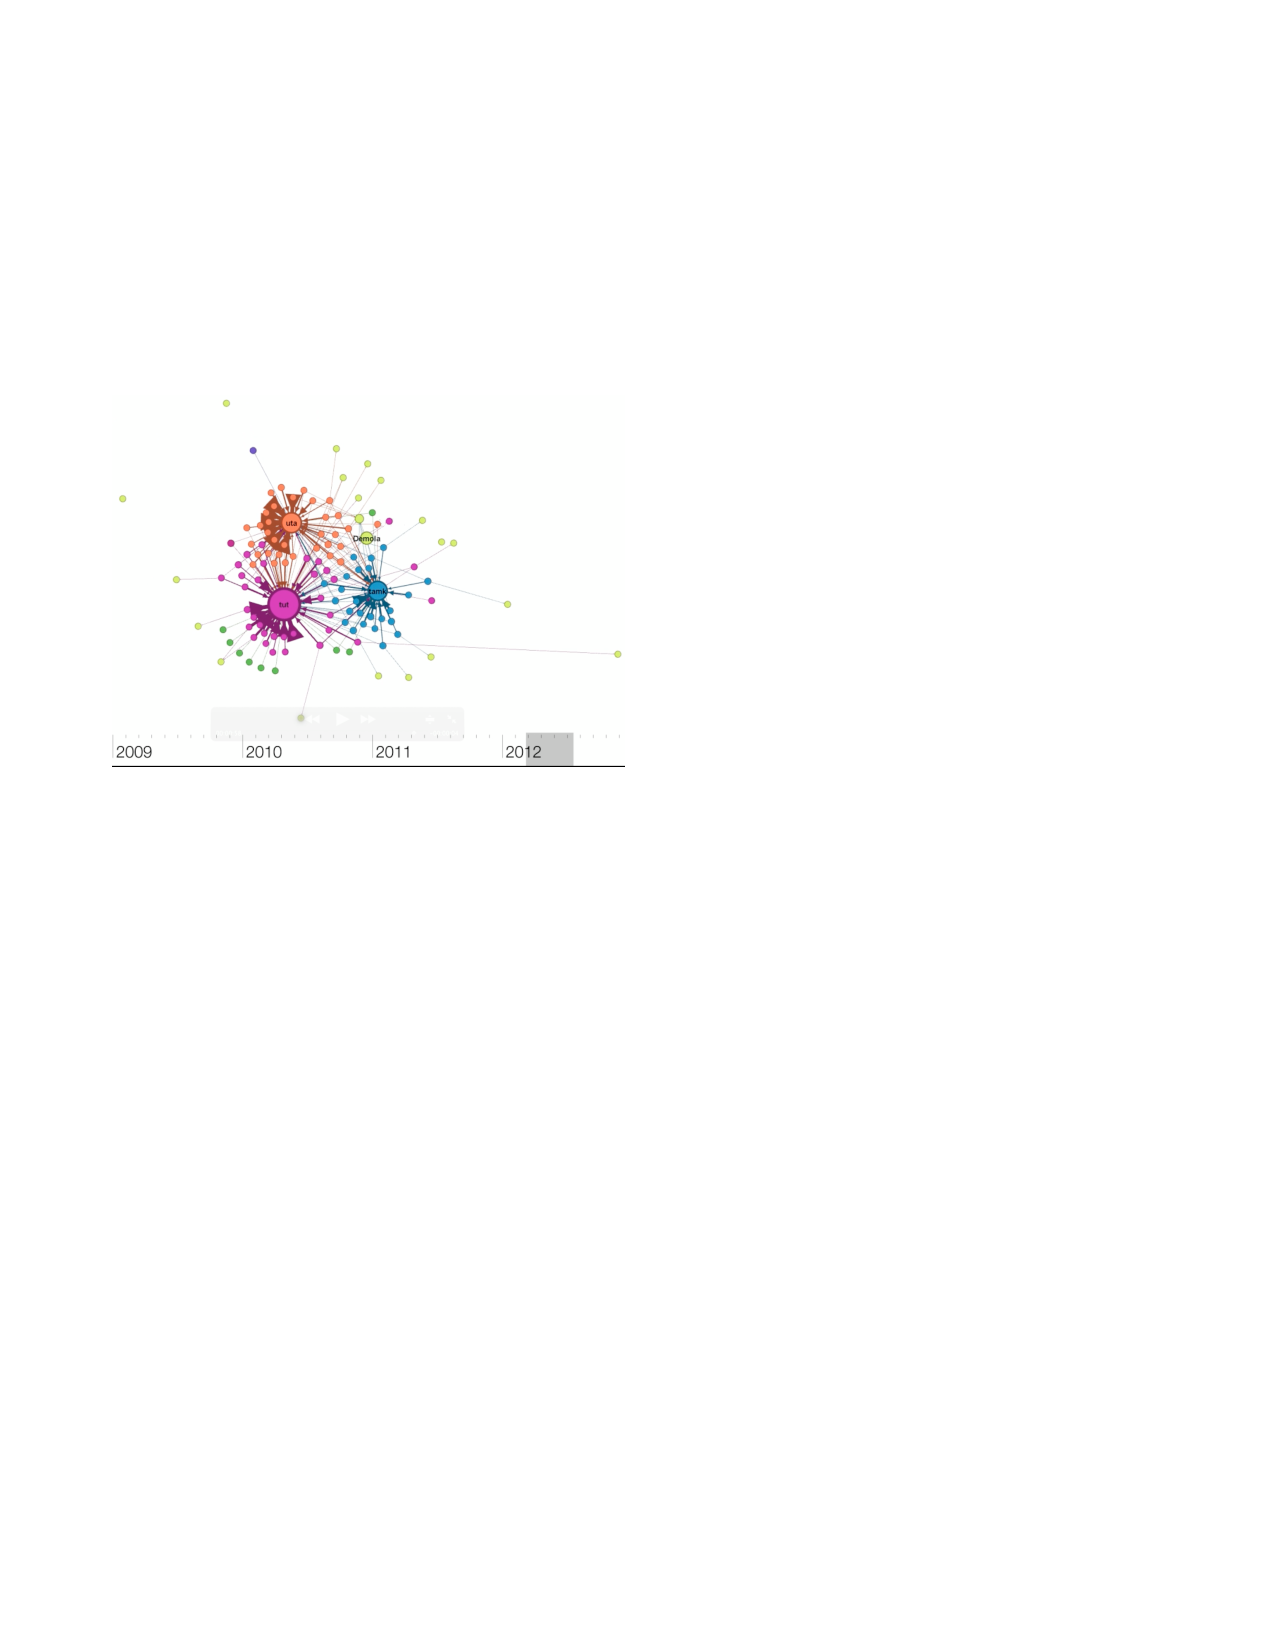
\includegraphics[width=12cm]{figure/Animating-Demola-Evolution.pdf}
\caption{Innovation platform Evolution: Animating Demola Evolution \citep{Huhtamaki2013ProcessDemola}}
\label{fig:animating-demola}
\end{figure}

Network Analysis and Visualization (NAV) process model \citep{Hansen2012DoData} is used to frame the analysis process. The implementation of the visualization process is an interplay between tailored code and the use of pre-existing tools. Python and NetworkX are used to pre-process the data and the visualizations and the animation are created with Gephi.

In network in Figure \ref{fig:animating-demola}, node size represents its betweenness value and edge weight shows the number of students affiliated with a particular university. Node colors represent network clusters. Force-driven algorithm is used to lay out the nodes. To show the dynamics of the Demola platform, edges connecting companies to individual projects only exist during the going of the project after which the layout algorithm starts pushing loose nodes away from the center. When force-driven layout is run in real time, the animation shows for example the retention patterns of individual companies engaging with the platform. Capturing of the video was done with a screen-recording software and timeline was included during post-production.

\subsection{Results and network-related insights}

The key output of the Demola investigation is the animation of the evolution of Demola Tampere Ecosystem from its first day of operation to the beginning of year 2013 when the investigation was conducted.

On basis of the feedback received both during the co-creation process as well as after the publishing the study, we claim that particularly the dynamic animation of the platform evolution is useful in presenting, describing, marketing and selling the platform for existing and new stakeholders. As evidence, we offer the fact that Demola operating team has continued to use the animated project network as a tool for communicating Demola activities and their evolution over time.

\section{Business domain level: mobile ecosystem}

The mobile ecosystem consists of a heterogeneous and continuously evolving set of companies that are interconnected through a complex, global network of relationships. There is however very little theoretical understanding on how these networks emerge and evolve and no well-established methodology to study these phenomena. Traditional approaches have primarily utilized alliance data of relatively established firms; however, these approaches ignore the vast number of relevant ecosystem activities that occur at the personal, entrepreneurial, and university level. In \cite{Basole2012UnderstandingApproach}, we argue and empirically illustrate that a data-driven approach can provide important complementary explanatory insights into the dynamics of the mobile ecosystem. We present our approach through two mobile ecosystem relationships that were formed just before the investigation--the strategic partnership between Nokia and Microsoft and Google’s acquisition of Motorola Mobility. Our analysis is complemented with network visualizations. The article concludes with implications and future research opportunities, some of which we ourselves took up in an extended version of the article \citep{Basole2015UnderstandingApproach}. 

This investigation was conducted without external stakeholders.

\subsection{Rationale for network analytics}
% * <jukka.huhtamaki@tut.fi> 2015-07-01T08:32:10.055Z:
%
%  Should we refer to analysis (rather than analytics) when we refer to individual analysis cases rather than the more general process used to conduct the individual analyses?
%

The investigation stems from the fact that there is very little theoretical understanding on how ecosystems emerge and evolve \citep{Ahuja2012TheNetworks}. Network modeling is an integral part of investigating ecosystems in system level. Companies, investors, and invididuals are represented as network nodes and their interconnections are tracked over time to analyze the emergence of ecosystem patterns. Snapshots of the structure are used to analyze the evolution of the structure. We admit that network analysis alone is not enough in developing rich insight on structures and mechanism underlying emergence and evolution and propose further investigations based on agent-based modeling \citep[cf.][]{Huotari2016WinnerMarkets}.  

\subsection{Data sources}

The ecosystems surrounding the pairs of companies are investigated with two complementing datasets. First, we use Thomson Reuters SDC Platinum, an institutionally curated dataset on deals and alliance between already established companies, for transactional microdata on the direct and second-tier connections of the pair of companies. Second, to add to the insights on startups and growth companies, venture capital investors and even key individuals, we tap into IEN dataset for complementary views into the ecosystem. IEN Dataset is a collection of socially constructed datasets on executives, finance, business angels and startups \citep{Rubens2010LeveragingMoves}.

\subsection{Network modeling decisions}

Figure~\ref{fig:mobile-ecosystem-sdc} shows the ecosystem surrounding Google and Motorola Mobility based on Thomson Reuters SDC data. In Figure~\ref{fig:mobile-ecosystem-iend}, the startup and growth company centric view of the ecosystem surrounding Google and Motorola Mobility is shown. Separate networks are created to represent ecosystem structure emerging from Thomson Reuters SDC (e.g. Figure~\ref{fig:mobile-ecosystem-sdc}) and IEN Dataset (e.g. Figure~\ref{fig:mobile-ecosystem-iend}). In previous, nodes represent companies and, in latter, companies, investors and individuals. In previous, companies are connected on basis of joint deals and alliances. In latter, companies are connected to investors, key individuals and other companies that have either acquired or invested in a company. 

\begin{figure}[htb]
\centering
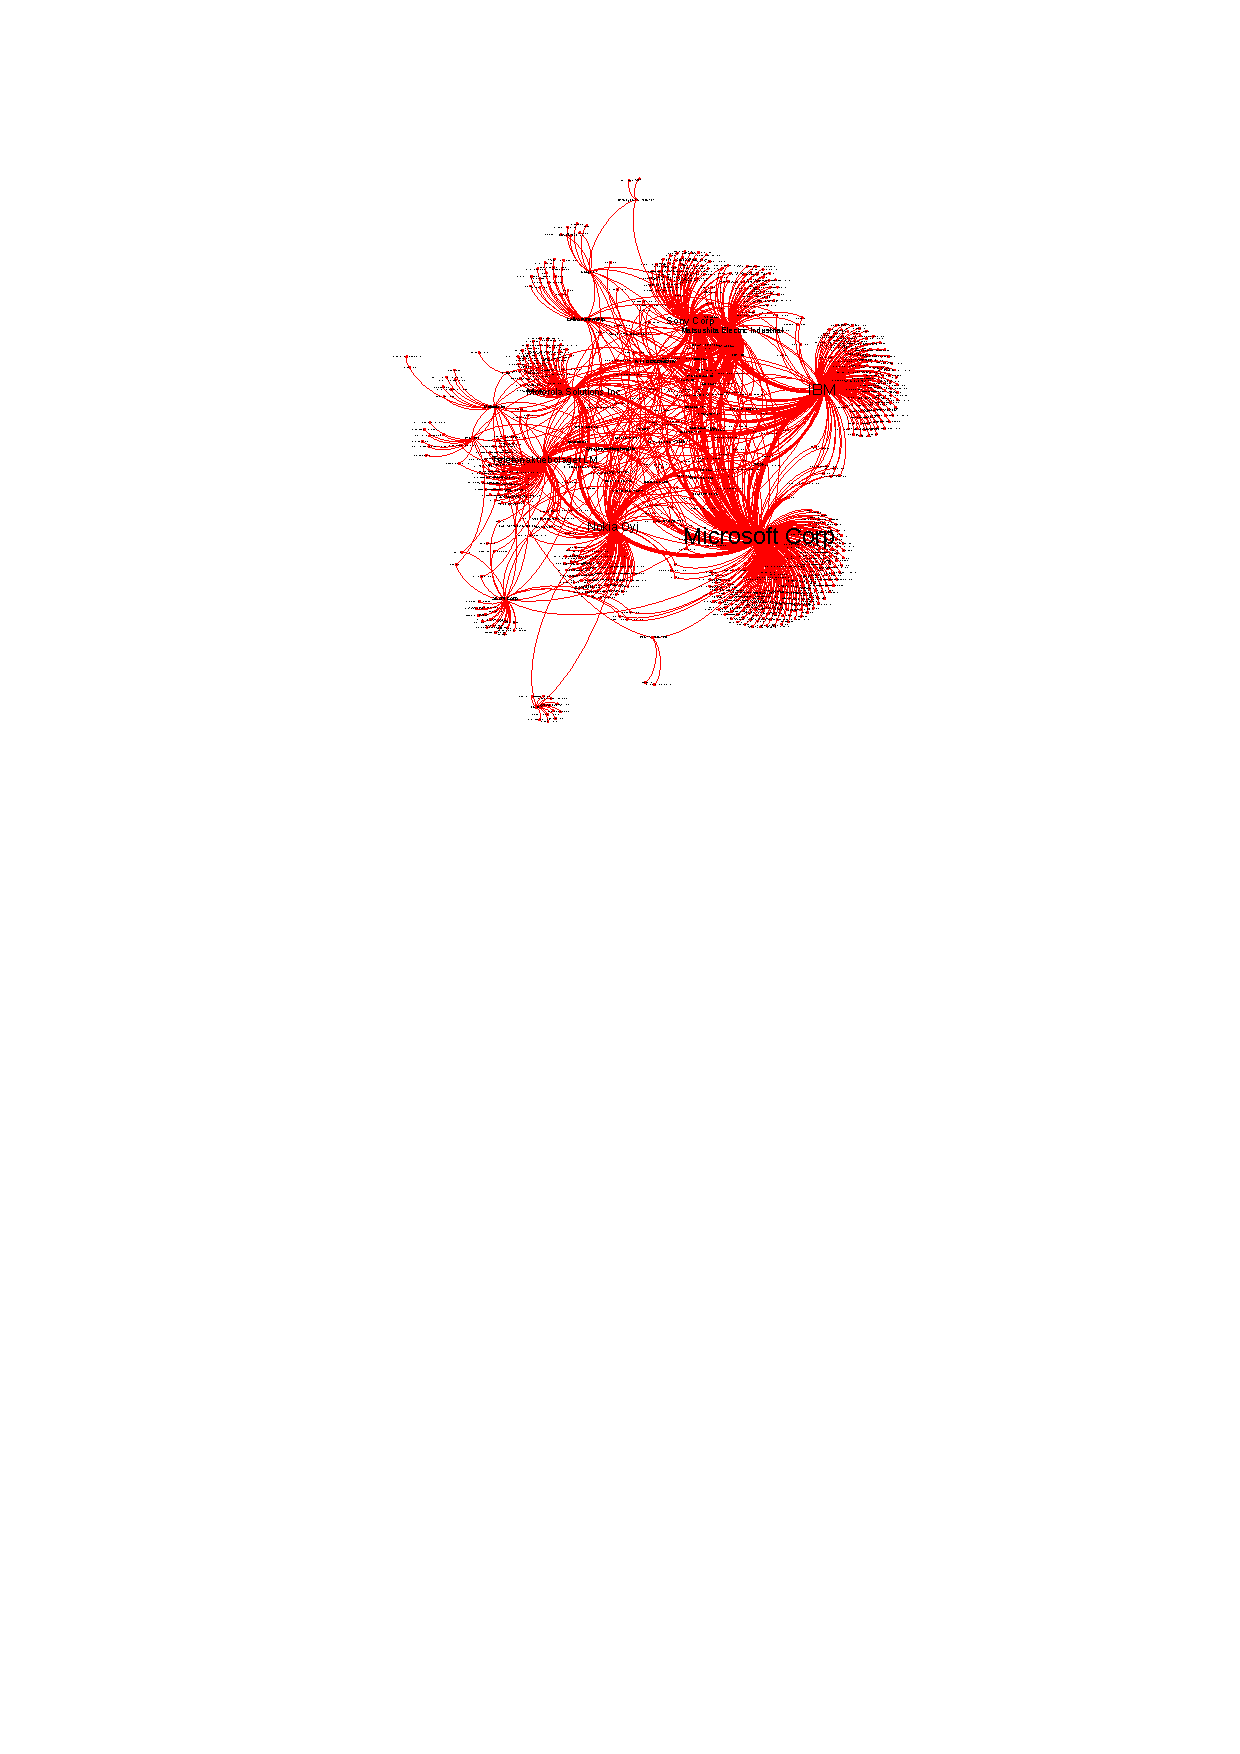
\includegraphics[]{figure/Mobile-Ecosystem-Google-Motorola-SDC.pdf}
\caption{Cumulative network around Google and Motorola Mobility using Thomson Reuters SDC data for deals and alliances. Through second-step connections, Microsoft becomes the key node in the network. \citep{Basole2012UnderstandingApproach}}
\label{fig:mobile-ecosystem-sdc}
\end{figure}

\begin{figure}[htb]
\centering
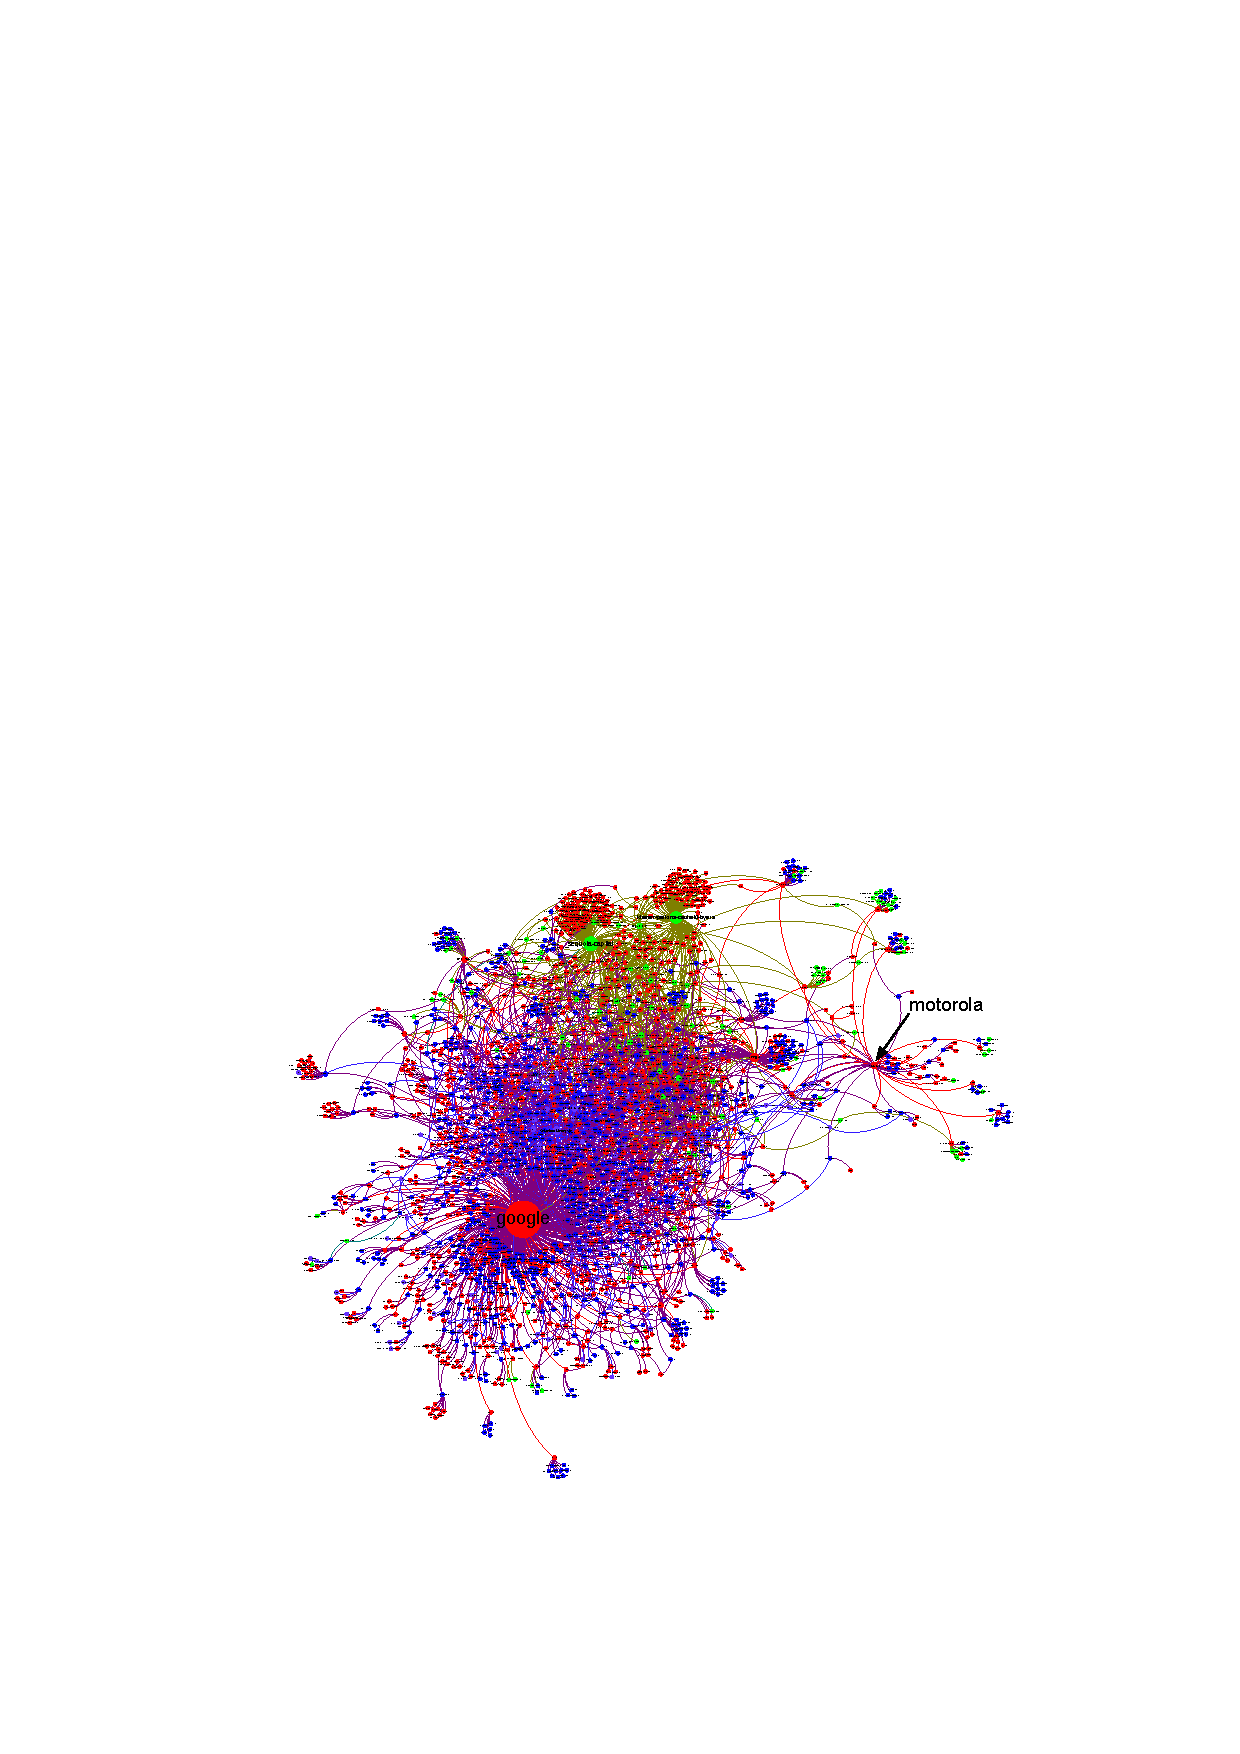
\includegraphics[]{figure/Mobile-Ecosystem-Google-Motorola-IEND.pdf}
\caption{Cumulative network around Google and Motorola Mobility. Google's approach to operating through acquisitions rather than deals and alliances (cf. Figure~\ref{fig:mobile-ecosystem-sdc}) is highlighted. \citep{Basole2012UnderstandingApproach}}
\label{fig:mobile-ecosystem-iend}
\end{figure}

Boundary specification includes the selection of nodes, node types and relationship types, analysis timeframe, as well as the steps from focal companies to include other companies and stakeholders \citep{Basole2012UnderstandingApproach}. In this investigation, all companies and other actors within two steps from the focal companies are included in the network. Force-driven algorithm is used to lay out the network.

For investigating the evolution of the structural properties of the ego-centric networks, we created snapshots of the networks and calculated the development of a set of node and network-level metrics over time. These measurements are represented as small multiples in the article.

\subsection{Results and network-related insights}

Two illustrative investigations exemplify the use of the data-driven approach for understanding the mobile ecosystem. In February 2011, Nokia and Microsoft announced a strategic alliance to work together in developing their mobile offering, both in terms of devices as well as an ecosystem feeding applications and other content to add value to device users. Google acquired Motorola Mobility in August 2011 to strengthen its capabilities in the mobile domain.

Separate network representations are created for the two set of data as well as the two cases. Figure \ref{fig:mobile-ecosystem-sdc} shows the 2-step network of Google and Motorola mobility with Thomson Reuters SDC Platinum data representing the ways that traditional enterprises operate. Even though not a focal company in this representation, Microsoft emerges as the supernode in the network. With network representation of IEN Dataset in \ref{fig:mobile-ecosystem-iend}, Google's true size accumulated particularly through series of acquisitions and the flow of talent is shown. 

\section{Program Level: Tekes Young Innovative Companies}

In \ref{pub:tekesyic}, we \citep{Huhtamaki2012NetworksFinland} explore a vital part of the Finnish innovation ecosystem: startups that are selected to Tekes Young Innovation Companies (YIC) program  for support in fast international growth. Highlighting the importance of networks, we proceed to analyze the existing relationships that these companies have with other companies, financing organizations as well as with individuals taking part in their co-creation. Moreover, we investigate the network of Twitter followers of the companies taking part in the YIC program for insights on the volumes of perception that the startups have accumulated.

The investigation was conducted as part of a Tekes-funded innovation research project on using social media data to measure innovation. The investigative team designed the data collection and network modeling process and interacted with Tekes representatives to fine-tune the parameters related to boundary specification and network modeling.

\subsection{Rationale for network analytics}

The companies are selected into the YIC program on basis of their individual properties through evaluation panels. In taking a data-driven approach into investigating the innovation ecosystem around these companies, our objective is to gain insights into the underlying structure in between companies and create a system-level view of the innovation ecosystem. 

We propose that these existing relationships in between startups may be used to make sense of companies' role as resource integrators within a network, contributing to its growth and success. Overall, we claim that network analysis and resulting network visualizations provide novel insights into the understanding of possibilities for global growth and success and, importantly, on the impacts of the YIC program in system-level.

\subsection{Data sources}

The list of startups participating in Tekes YIC program is scraped from Tekes homepage\footnote{Startups at the Tekes Young Innovative Company programme, \url{http://www.tekes.fi/en/funding/yic/companies/}}. Innovation Ecosystems Network Dataset \citep{Rubens2010LeveragingMoves} is used for data on  companies, investors, key individuals and acquisitions. 

Moreover, Twitter usernames of the YIC companies are compiled into a spreadsheet in a semi-manual manner and a tailored script is implemented to crawl Twitter REST API\footnote{Twitter Developers: REST APIs, \url{https://dev.twitter.com/rest/public}} to collect the list of followers for each YIC company with a Twitter account.

\subsection{Network modeling decisions}

For boundary specification, startups taking part in the Tekes YIC programs are used as focal points in the network in Figure~\ref{fig:tekes-yic-3-step}. All the investors that have invested into the companies in Tekes YIC program are included, as well as all the individuals that, according to IEN dataset, are affiliated with the companies. In addition, to explore the larger context of the companies in YIC, all the other companies that the individuals are or have been affiliated with are included in the network. Companies in the Tekes YIC program are represented as light blue nodes, other companies are red, individuals blue and investors green. Node size represents its betweenness centrality to highlight the key nodes in bridging the different parts of the network. Finally, the network is laid out with a force-directed algorithm.

\begin{figure}[htb]
\centering
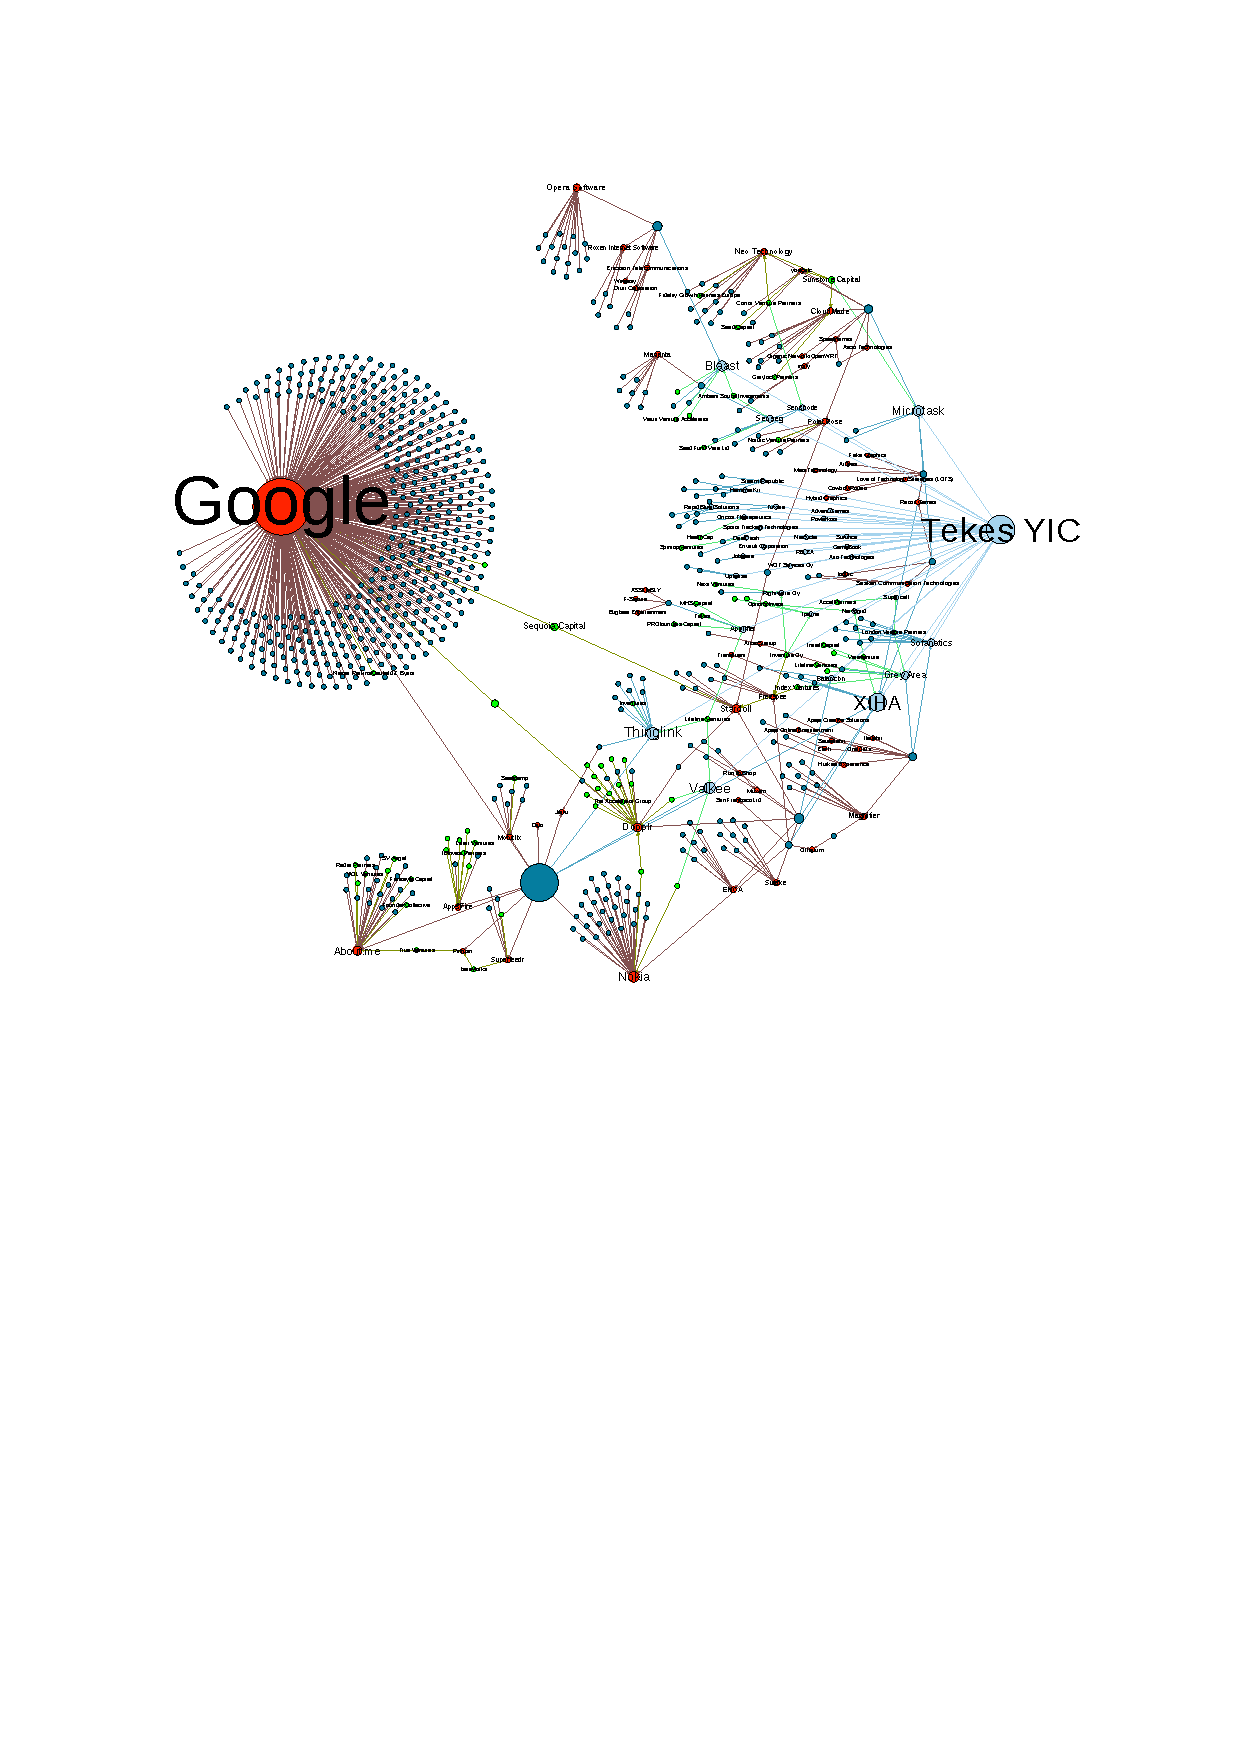
\includegraphics[width=12cm]{figure/Tekes-YIC-3-step.pdf}
\caption{Boundary specification: 3-step network visualization of Tekes Young Innovative Companies, their direct connections and the companies, investors and individuals that can be reached through the direct connections
 \citep{Huhtamaki2012NetworksFinland}}
\label{fig:tekes-yic-3-step}
\end{figure}

\begin{figure}[htb]
\centering
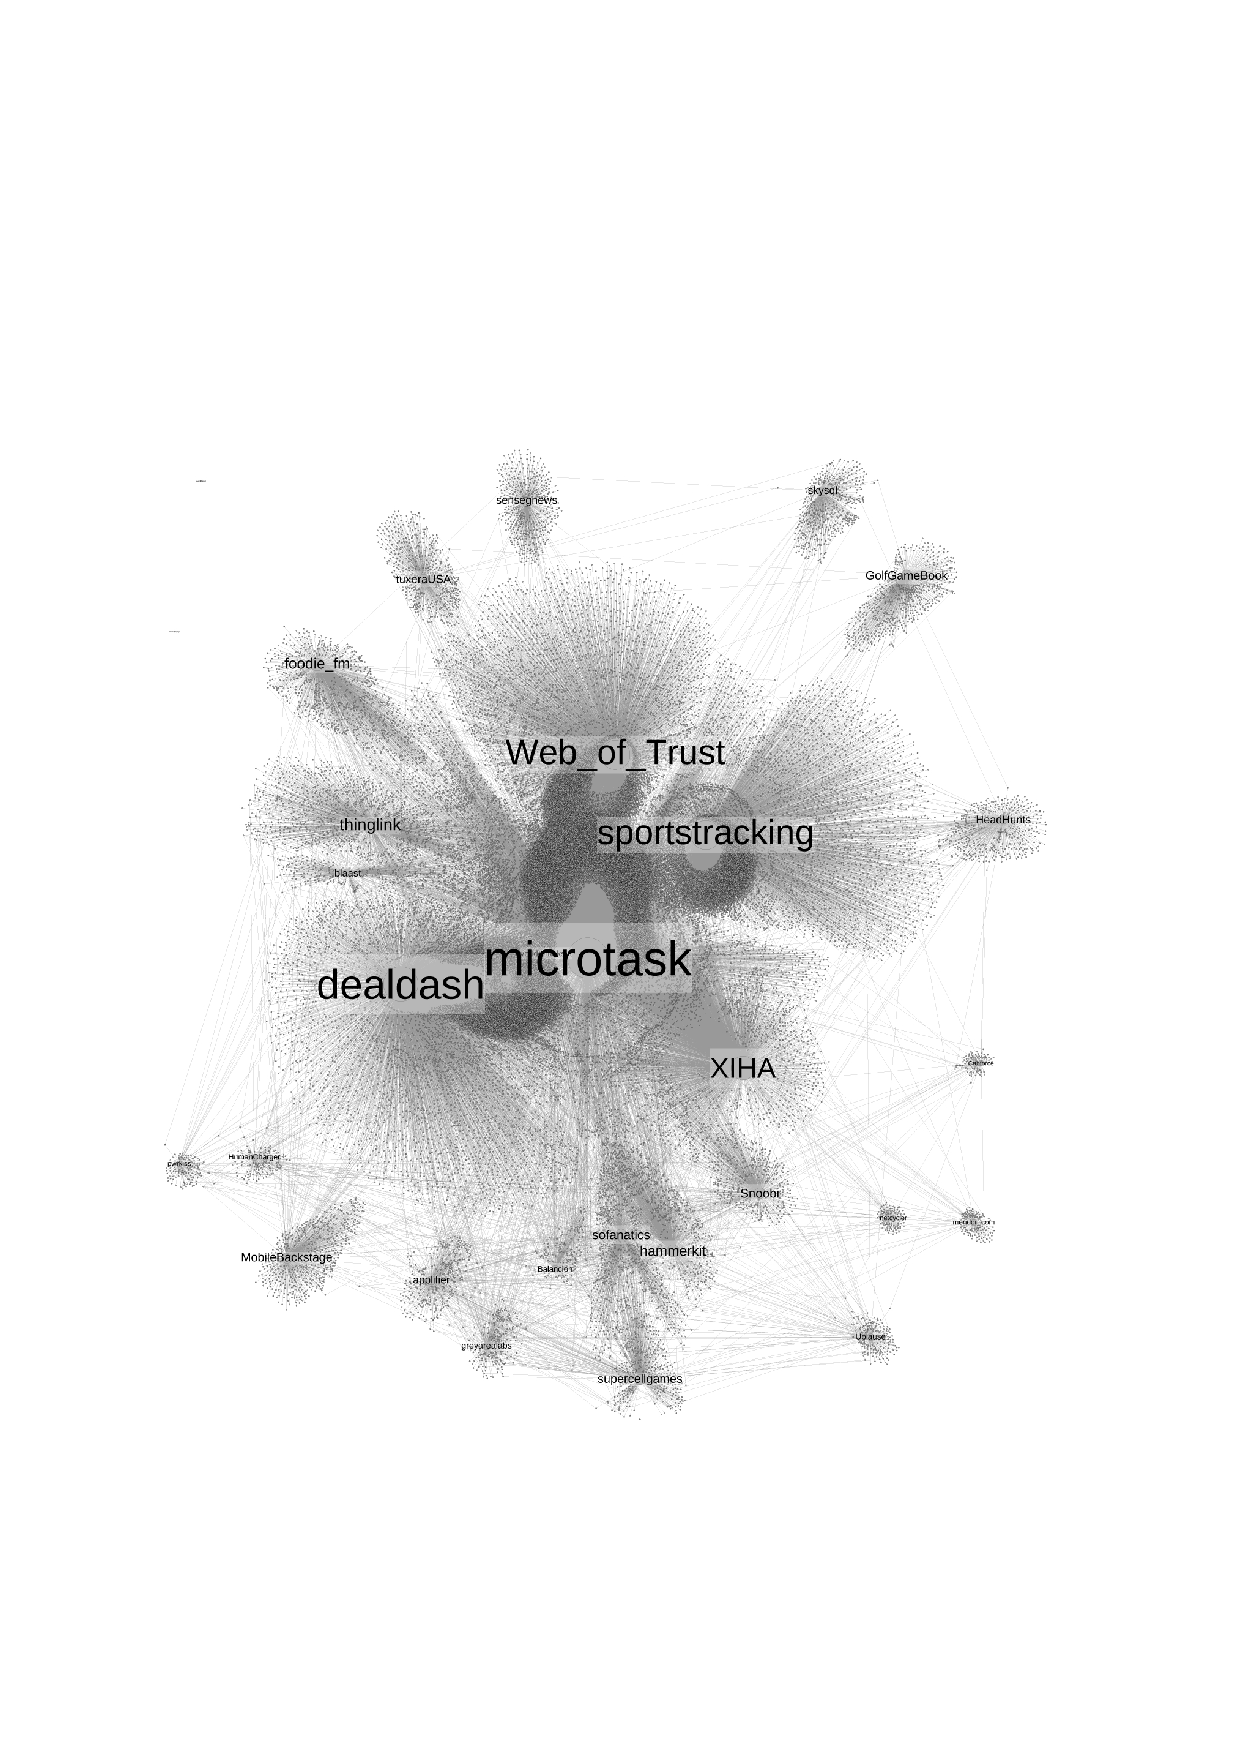
\includegraphics[width=12cm]{figure/Tekes-YIC-Twitter.pdf}
\caption{Social media analytics: 3-step network visualization of Tekes Young Innovative Companies, their direct connections and the companies, investors and individuals that can be reached through the direct connections
 \citep{Huhtamaki2012NetworksFinland}}
\label{fig:tekes-yic-twitter}
\end{figure}

In the Twitter network in Figure~\ref{fig:tekes-yic-twitter}, all the followers of a company are connected to the company with a directed edge pointing toward the company. The result is a two-mode or bipartite directed dichotomous network. Node size represents it indegree. Force-driven layout algorithm is used the lay out the Twitter network.

\subsection{Results and network-related insights}

The intestigative team joined with Tekes YIC program representatives for sensemaking to identify the key insights. With the first steps of connecting investors and individuals, it becomes evident that the companies selected individually into the Tekes YIC program are not without interconnections. When adding another step, the companies connected to the YIC program indirectly through investors or individual people are included and additional connecting tissue is introduced. Both Google and Nokia get pulled in through second-step connections and a single individual becomes a bridge between Nokia and Google and therefore has the largest betweenness value.

With ground truth, we know that an early social media platform Jaiku is one of the key individual developments in the Finnish Innovation Ecosystem. After Google acquired Jaiku, its founders Jyri Engeström and Petteri Koponen continued their ventures, Engeström as a serial entrepreneur in San Francisco Bay Area and Petteri Koponen through  Lifelines Ventures he co-founded. Interestingly, Lifeline Ventures is one of the early investors into Supercell, the most recent success story of the Finnish innovation ecosystem. More recently, Supercell CEO Ilkka Paananen joined the advisors of Lifeline Ventures to support the creation and growth of new startups.

Microtask, Web of Trust, Sportstracking and DealDash form the core of the Tekes YIC startup follower network. Microtask leads the charts with more than 30,000 followers followed by DealDash and Web of Trust. Supercell (\href{https://twitter.com/supercellgames}{@supercellgames}) has less than 1000 followers during the time of the investigation. In May 2016, more than 280,000 Twitter users follow Supercell.

\section{National level: Finnish Innovation Ecosystem}

Finnish Innovation Ecosystem is investigated in two consecutive experiments presented in \ref{pub:finland} and \ref{pub:multiscopicfinland}. Out of all the experiments included in this dissertation, \ref{pub:finland} is the first we \citep{Huhtamaki2013AFinancing} conducted\footnote{The paper on the investigation was first presented in EBRF conference in 2010 and invited to be published in TIM Review, see \url{http://timreview.ca/article/424}, and was eventually selected to book Value Co-Creation: Best of TIM Review.}. Therefore, its main contribution is in serving as a stepping stone for further investigation. 

In \ref{pub:multiscopicfinland}, we \citep{Still2013NetworksFinland} take up a grand challenge to present a solution for modeling and visualizing the network structure of the innovation ecosystem of a single nation, here Finland. To create a system-level view on Finnish Innovation Ecosystem, we utilize three complementary sources of data, each representing different aspects of the ecosystem.

We resolve the limitations of the separate datasets by building multiscopic views into networks of innovation relationships, using separate datasets. Moreover, in order to create an system-level view into Finnish Innovation Ecosystem, we create an aggregated dataset by combining the three individual sets of data. We proceed to support the interpretation of these visualizations by explaining context with network metrics as well as other descriptions.

The two investigations on the Finnish Innovation Ecosystem are conducted in innovation research projects funded by Tekes innovation research. The investigative team conducted the investigations independently, however project steering group members representing Finnish innovation ecosystem stakeholders had a role in formulating the research questions guiding the studies.  

\subsection{Rationale for network analytics}

Investigation of the Finnish Innovation Ecosystem is an attempt to utilize the potential of the data-driven approach to network analytics in the level of a national ecosystem. It stems from the observation  that traditional ways to measure innovation inputs and outputs are often industry-level aggregates and therefore do not allow for system-level insights on the innovation ecosystem under investigation \citep{Still2012ParadigmDigital}. Network representation of a national innovation ecosystem allows for observing e.g. the role of individual investors and patterns of acquisition and workforce flow and, in addition, developing a context for measurements and tailored action. More importantly, ecosystem-level view enables co-referencing and therefore more explicit support for sensemaking and attempts to form shared vision in between ecosystem stakeholders \citep{Russell2011TransformingOrchestration}. To recap, the presented multiscopic views into the Finnish Innovation Ecosystem allows for examining the relationships supporting value co-creation at various levels of the ecosystem as well as between those levels, providing novel possibilities for network orchestration and innovation management.

\subsection{Data sources}

Three complementary sets of data are used in the investigation. Thomson Reuters SDC includes in particular connections in between large, already established companies. In addition, to enable the investigation of the relationships around startups and growth companies, we use IEN Startup and IEN Growth to complement the analysis. More specifically, IEN Startup is used to create the microscopic view, IEN Growth the mesoscopic view and Thomson Reuters SDC the macroscopic view.

In addition to using the three sources of data in parallel, an aggregate dataset is created. The three datasets in use in the investigation are complementary and, at the same time, partly overlapping, therefore necessitating a refinement and curation process similar to what is being applied e.g. in data journalism \citep[cf.][]{2012DataHandbook} when creating the aggregated dataset.

\subsection{Network modeling decisions}
\begin{figure}[htb]
\centering
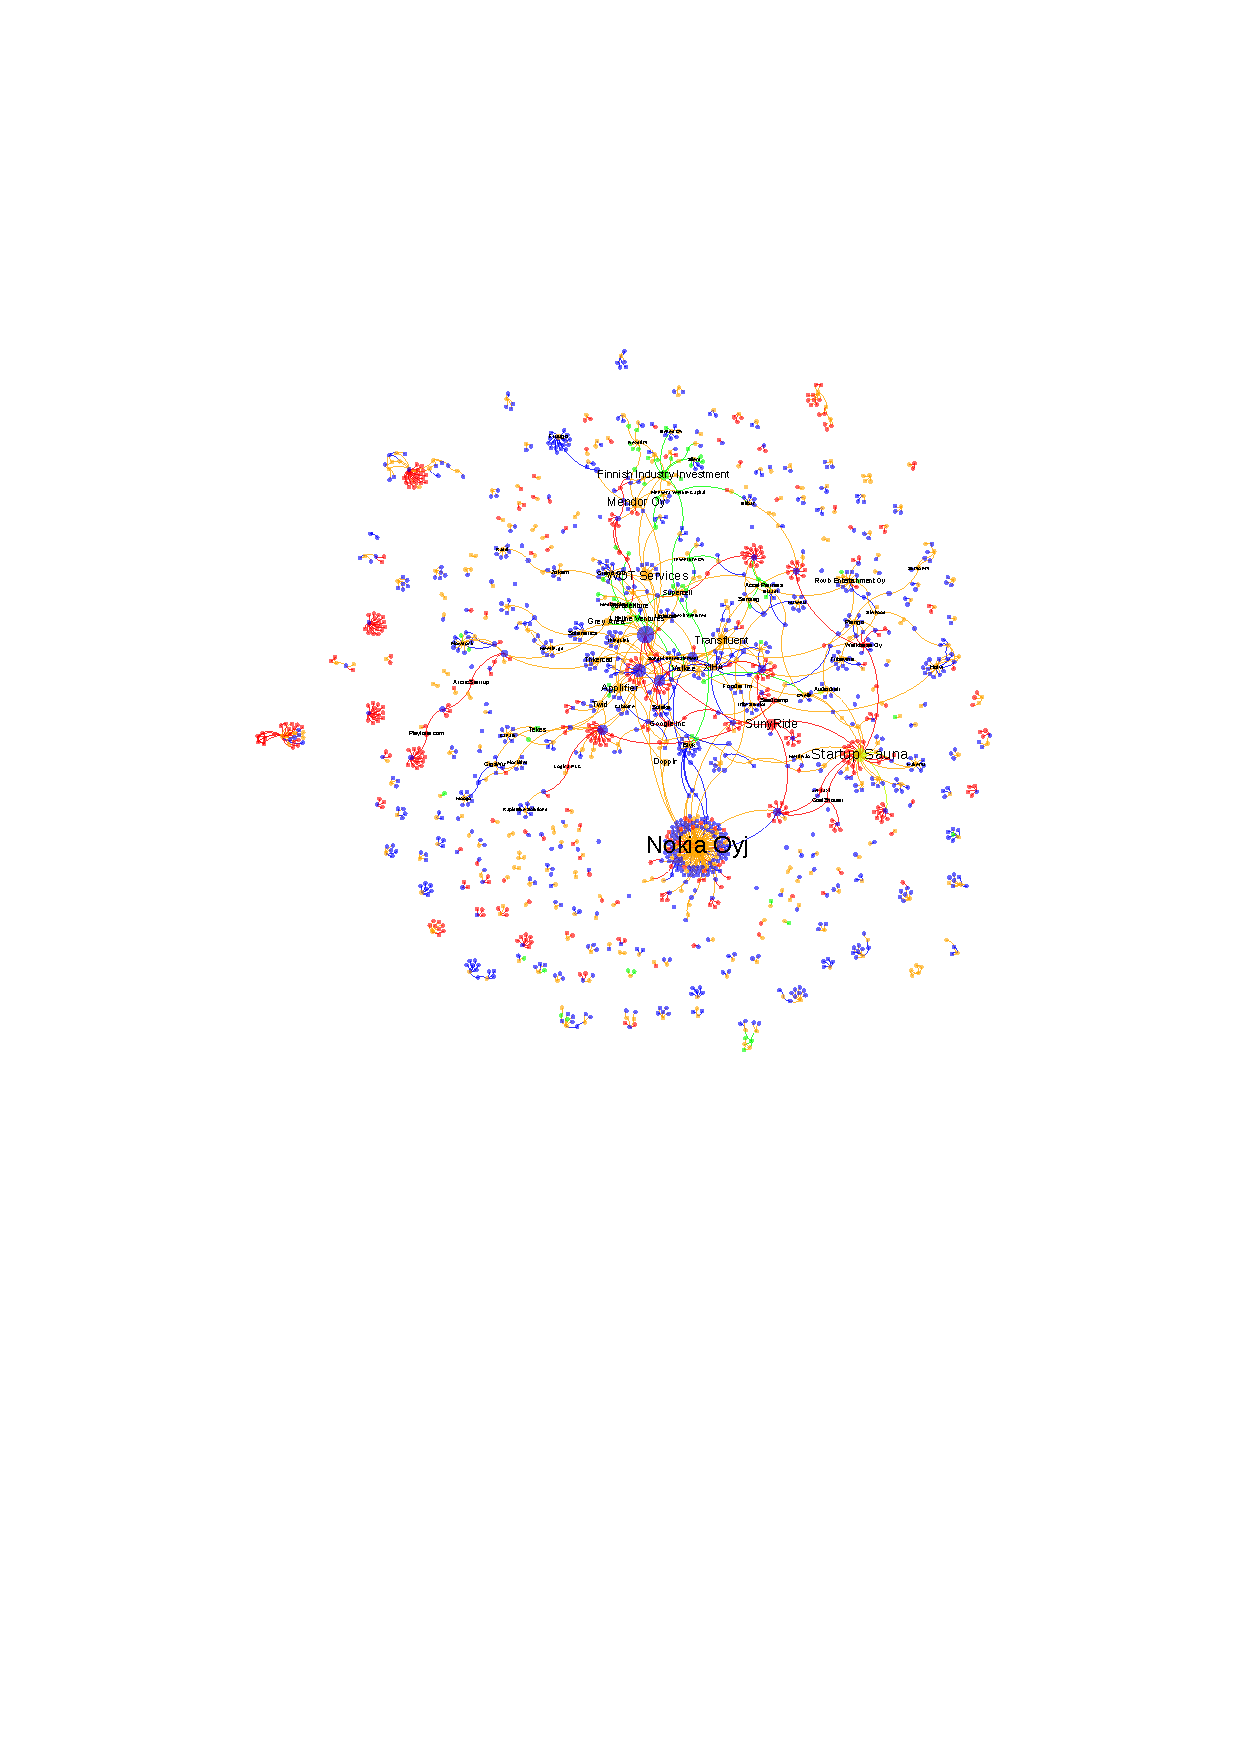
\includegraphics[]{figure/Finland-Multiscopic.pdf}
\caption{Data aggregation: Aggregate view to the Finnish Innovation Ecosystem using data on deals and alliances, executives and finance, and business angels and startups  
\citep{Still2013NetworksFinland}}
\label{fig:finland-multiscopic}
\end{figure}

\ref{pub:multiscopicfinland} is the first investigation in which we provide a multiscopic view into an innovation ecosystem, in this case the Finnish innovation ecosystem. In all, four different views into the Finnish Innovation Ecosystem are created. Macroscopic view shows the connections in between already established enterprises. Finnish companies are included and connected to other companies, Finnish or foreign, through deals and alliances. Mesoscopic view is built around Finnish growth companies. All the organizational investors as well as key individuals affiliated with the companies are included and connected to the Finnish companies. Microscopic view includes Finnish startups as well as business angels and other seed level investors and individual people affiliated to the companies. Multiscopic view, an aggregate of the three levels, provides a holistic system-view into the Finnish innovation ecosystem. 

To complement the multiscopic views into the Finnish Innovation Ecosystem, a number of quantitative descriptions for the different network representations is included in the article. These include the number of nodes, number of connections, density and diameter. Moreover, we list the top 10 actors based on betweenness centrality and degree for each of the networks.

\subsection{Results and network-related insights}

The main results of the investigation is the multiscopic view into the Finnish Innovation Ecosystem in Figure \ref{fig:finland-multiscopic}. The aggregated network depicts an ecosystemic view of Finland in Figure \ref{fig:finland-multiscopic} as it combines the Finnish companies from the three separate datasets and shows their direct connections. Hence, for the first time, we can see a single network representation of an ecosystem of the founders and angels, executives and financing organizations, as well as companies from startups to established enterprises. Overall, key actor of the ecosystem with the highest betweenness centrality is not surprising: Nokia is the super-node due to its connecting role in the Finnish ecosystem. % Accordingly, the same companies, financing organizations and individuals that have been prominent in previous lists and visualizations are highly visible in this ecosystemic view. 
As the weight of micro and meso-level data is greater, the top ten list of actors in the multiscopic level on basis of both betweenness and degree includes a significant number of individuals. There are 7 shared nodes between micro and macro-level views; 184 between micro and meso-level views; 10 between meso and macro-level views; four nodes appear in all three views: Rovio Entertainment, F-Secure, Mendor and Nokia. A number of foreign companies are included in the network through second-step connections, e.g. through acquisitions, investors, or individuals affiliated with Finnish companies.

\section{International level: EIT ICT Labs}

The network structure of EIT ICT Labs innovation ecosystem is investigated in \ref{pub:eitictlabs} \citep{Still2014InsightsVisualisations}. EIT ICT Labs, rebranded as EIT Digital \footnote{EIT ICT Labs becomes EIT Digital, \url{https://www.eitdigital.eu/news-events/news/article/eit-ict-labs-becomes-eit-digital/}} in June 2015, is a ``Leading European open innovation organisation.'' 

The investigation presented in \ref{pub:eitictlabs} builds heavily on \cite{Still2012ParadigmDigital} with an objective to explore opportunities for supporting the orchestration of innovation ecosystems, hence contributing to a fundamental capability in the networked world. We use a data-driven, relationship-based and network centric approach to operationalize Innovation Ecosystems Transformation Framework (IETF) \citep{Russell2011TransformingOrchestration} and present analysis, evaluation and interpretation in order to provide decision support and insights for transforming innovation ecosystems.

The investigative team joined with representatives of EIT ICT Labs Helsinki co-location center to conduct the two investigations \citep{Still2012ParadigmDigital, Still2014InsightsVisualisations}. In addition to mapping the network structure of EIT ICT Labs, the investigative team took up a scenario planning experiment that emerged trough interaction with EIT ICT Labs representatives to as a what-if question: What if San Francisco Bay Area was the seventh node of EIT ICT Labs? 

\subsection{Rationale for network analytics}

We investigate how data-driven network visualizations can be used to produce insights that support innovation ecosystem orchestration. The goal of network orchestration is a guided transformation of the ecosystem with continuous co-creation that allows the evolution of the processes needed to motivate and realize the transformation \citep{Russell2011TransformingOrchestration}. This process evolution accommodates the complex influences on innovation in a networked world and energizes innovation processes and outcomes. Through the lens of the IETF, a shared vision of the transformational potential of a dynamic innovation ecosystem is created through changes in actors, the events that they enable and the coalitions reflected in their relationships.

\subsection{Data sources}

After experimenting with in-house data on EIT ICT Labs activities, the investigative team together with EIT ICT Labs representatives decided to use IEN Dataset instead. The use of an external data source enables the  exploration of existing pathways in between the EIT ICT Labs co-location cities previously unknown to EIT ICT Labs operating team.

Innovation Ecosystem Network Dataset \citep{Rubens2010LeveragingMoves} is used as the sole data source. The dataset for the EIT ICT Labs sample is drawn by selecting all the companies that have their primary office in one of the six co-location cities of EIT ICT Labs: Berlin, Eindhoven, Helsinki, Paris, Stockholm, and Trento. In addition, to collect data representing companies and related individuals and investors in the SF Bay area, we listed all the key cities located in Silicon Valley area and complemented the list with San Francisco (including e.g. Berkeley).

\subsection{Network modeling decisions}

\begin{figure}[htb]
\centering
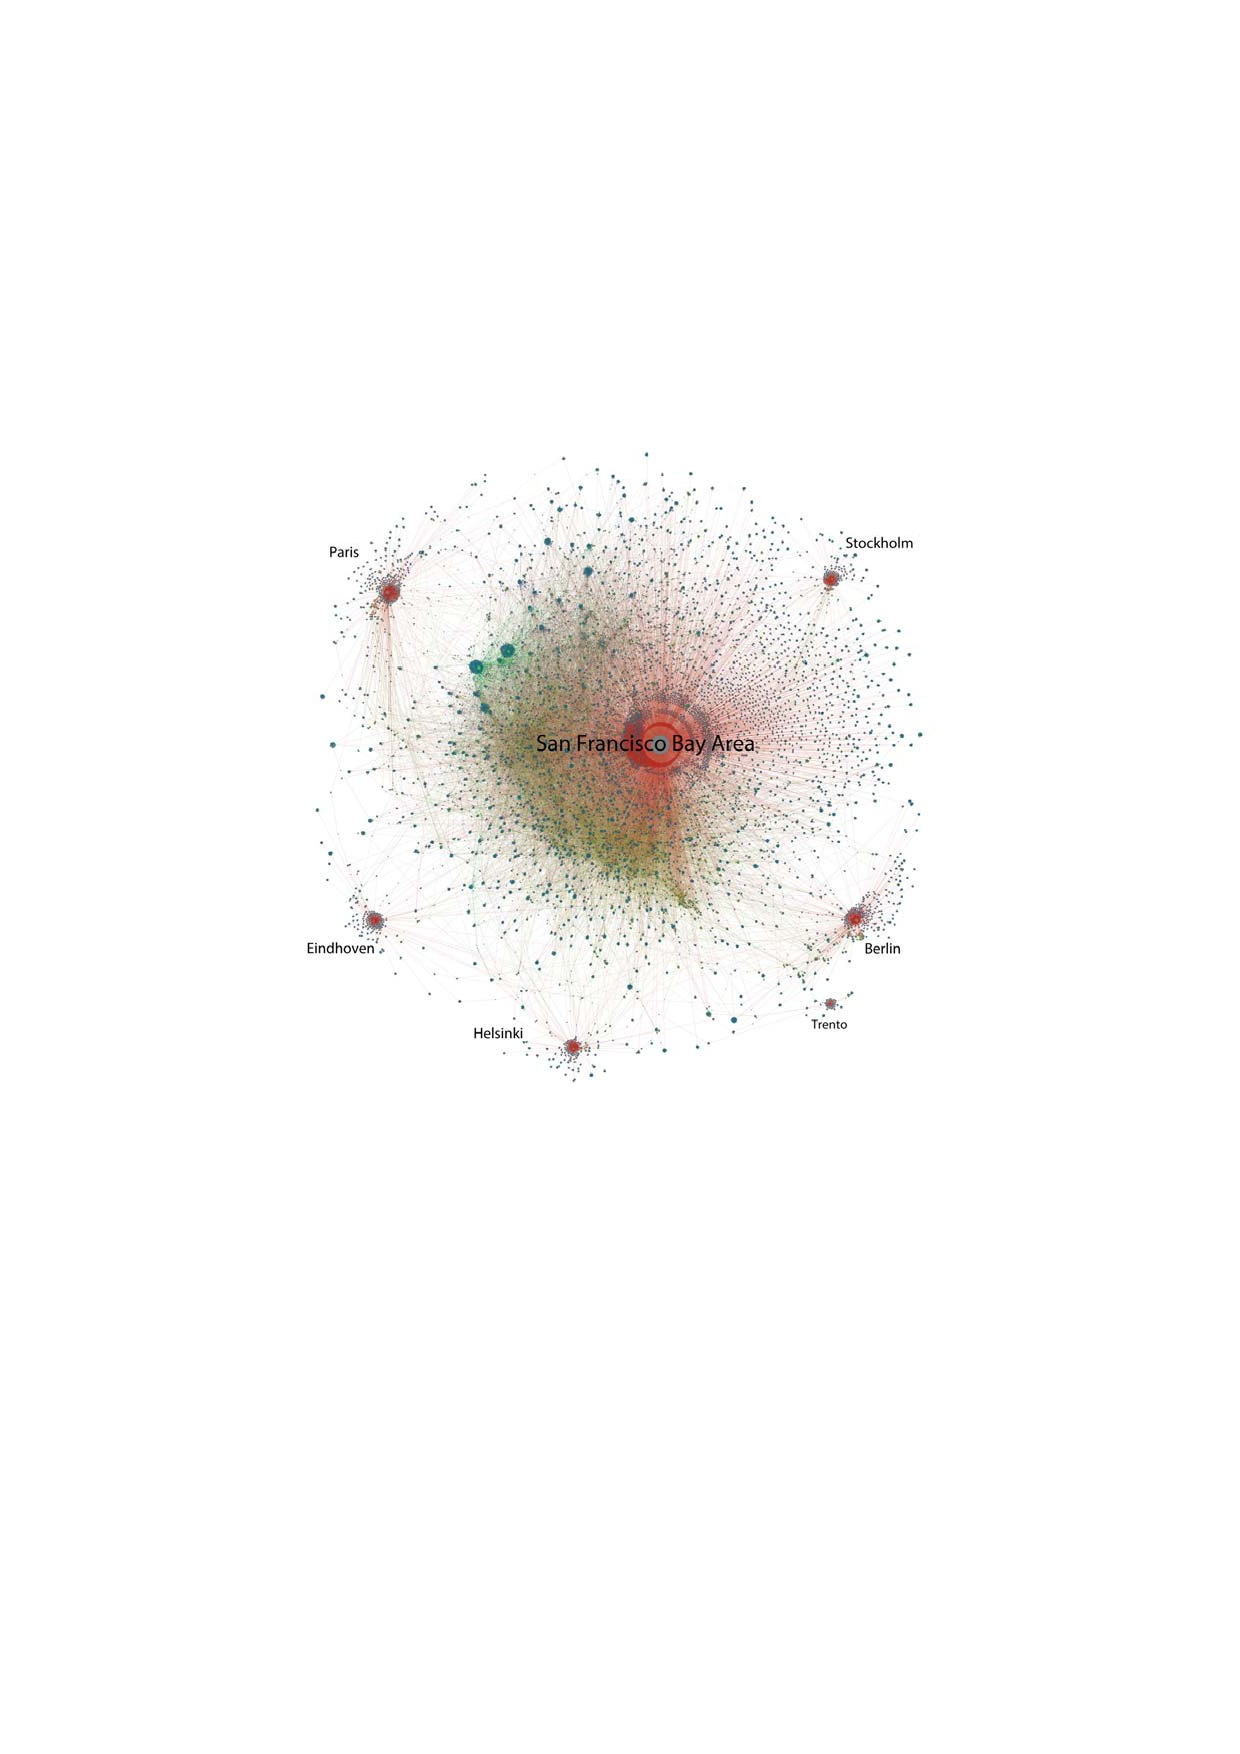
\includegraphics[width=0.925\textwidth]{figure/EIT-ICT-Labs-What-if-SF-Bay.pdf}
\caption{Scenario planning: What if San Francisco Bay Area was the 7th EIT ICT Labs co-location city \citep{Still2014InsightsVisualisations}}
\label{fig:eit-ict-labs-SF-Bay}
\end{figure}

The six co-location cities, Paris, Berlin, Stockholm, Helsinki, Eindhoven, and Trento, form the core of the network. Each company in the sample is connected to the city in which its primary office is located. All key individuals (founders, board members and C-level executives) in the dataset affiliated with one or more of the companies in the sample are connected to the companies. Next, financial organizations identified with funding events for those companies are added as nodes and connected to respective companies. 

Metrics used in the analysis include the number of each type of actors and the changes in the values over years 2011, 2012, and 2013. Moreover, we measure the degree and betweenness of the six co-location cities and the change in the values between 2012 and 2013 to investigate the changes in the relative position of the co-location cities.

\subsection{Results and network-related insights}

The results of the investigation include changes in the numbers of actors connected individual co-location cities compared to our previous investigations and a set of visualizations on the structure of the EIT ICT Labs ecosystems. Moreover, the role of individuals and investors in building interconnections between EIT ICT Labs co-location cities is shown. 

The prominent role of investors as the connecting tissue between the individual co-location cities is a key result of the investigation. Moreover, the realization that many of these investors are, in fact, based in Silicon Valley led us, in collaboration with EIT ICT Labs representatives, to ask a key what-if question: What if San Francisco Bay Area was the 7th EIT ICT Labs co-location city? Figure \ref{fig:eit-ict-labs-SF-Bay} shows that when San Francisco Bay Area is added as the 7th co-location city and the network representation is laid out with force-driven algorithm, San Francisco Bay Area becomes the focal point of the network through which most of the connections between the current co-location cities go through. With San Francisco Bay Area, the amount of nodes increases from 6,187 to 35,389 and edges from 7,050 to 51,106.

\section{Summarizing the investigations}

We will conclude this chapter with a summary of the results and network related insights into the investigated innovation ecosystems. Finally, we will discuss the utility and added value of the investigations.

For the investigation on Demola, we joined with the Demola operating team to explore ways to apply data-driven visual network analytics in representing the structure and dynamics of an ecosystem engager that is targeting to facilitate collaboration between (Tampere-based) universities and companies. In collaboration, i.e. through the process of guided emergence, we found an animation of the evolution of the network structure of Demola platform to be particularly useful in presenting, describing, promoting, and marketing the platform for existing and new stakeholders.

In the investigation on Tekes Young Innovative Companies, we explored the interconnections in between companies taking part in the YIC program. Two sources of data were used to conduct the study, Innovation Ecosystem Network Dataset and Twitter. We show that connections exist in between the companies that are individually selected into the YIC program. These interconnections are key in revealing the innovation ecosystem that Tekes is interacting with through their support for individual companies. Moreover, the investigation makes a contribution with an example of using social media data to give a system-level view into those interested in the companies. On a longer term, should the Tekes YIC program be successful in selecting and supporting companies in growing, we would see a food chain of investors and acquirers emerge. Business angels, serial entrepreneurs--either active or successful--would also take a central role in such a network representation of the innovation ecosystem around the YIC program. 

In the investigation of the Finnish Innovation Ecosystem, we provided a system-level view into a national innovation ecosystem. The ecosystem representation includes established enterprises, growth companies, and startups as well as investors and key individual affiliated with the companies. More specifically, we create four different representations of the ecosystem, microscopic, microscopic, macroscopic and multiscopic. A handful of key individuals that entered the global startup ecosystem early and were successful in growing and selling a company maintain a prominent role in the Finnish Innovation Ecosystem. Nokia is visible through its role as a source of talent flowing into the ecosystem. Startup Sauna, a student-driven accelerator\footnote{Startup Sauna accelerator is ``Building a better startup ecosystem one company at a time'', \url{http://startupsauna.com/}},  also has a notable role. Recent success stories Rovio Entertainment and Supercell take a peripheral position; the presented approach does, however, enable monitoring the evolution of the ecosystem around them in the future. Our practical suggestions for startups include active communication and data sharing using a wide variety of media and, particularly for policy makers, the utilization of network views for targeted actions as well as for creating shared understanding and vision.

From network orchestration viewpoint, in collaboration with EIT ICT Labs representatives, our results indicate that with coordinated and continuously improved use of visual and quantitative social network analysis, special characteristics, significant actors and connections in the innovation ecosystem can be revealed to develop novel insights. Creating a network representation of EIT ICT Labs including San Francisco Bay Area as the 7th node is an example of scenario planning that the approach proposed in this dissertation enables. We conclude that the IETF transformation framework can be used to develop shared vision and to support the orchestration of innovation ecosystem transformations.

\section{Utility and added value of the investigations}

In summarizing the approach and key findings of our first investigation on EIT ICT Labs \citep{Still2011ExplainingEurope}, \cite{Turpeinen2011}, EIT ICT Labs Helsinki co-location lead at the time and our collaborator in the investigation, pointed out the key role of mobility in EIT ICT Labs' attempt to turn Europe into an equal competitor to Silicon Valley. While EIT ICT Labs' key way to support mobility was at the time the European-level master school, the network representation of the interconnections between EIT ITC Labs co-location cities provided an interesting insight: the role of individual universities and in particular venture capital investors in bridging the co-location cities is very important. When revisiting investigation on EIT ICT Labs \citep{Still2012ParadigmDigital, Still2014InsightsVisualisations}, we joined with EIT ICT Labs representatives to ask a what-if question, something that is seen integral in scenario planning \citep{Schoemaker1995ScenarioThinking}.

In light of our investigations, we were exited to witness the news of, first, EIT ICT Labs opening up an office in San Francisco for ``Building a bridge between the European ecosystem and the San Francisco Bay Area''\footnote{EIT ICT Labs opens new Silicon Valley Hub, \url{http://eit.europa.eu/newsroom/eit-ict-labs-opens-new-silicon-valley-hub}} and, second, Marko Turpeinen appointed to lead the Silicon Valley Hub\footnote{Marko Turpeinen to lead EIT ICT Labs Silicon Valley Hub,  \url{http://www.aalto.fi/en/current/news/2015-04-29-002/}}. While the specifics of the decision-making process related to these two events remain unknown to us, we argue that the process related to the what if-scenario as well as the exploration of the structure of the existingecosystem in general contributed and supported discussions and decision-making related to  EIT ICT Labs' presence in Silicon Valley.

The Demola investigation was conducted during the time when the Demola concept was only beginning to grow outside Tampere and Finland. Similarly to the investigation on EIT ICT Labs, our co-creators in the Demola investigation knew the Demola operations by heart and therefore saw no value in exploring the structure of the Demola network for supporting their internal operations and decision-making. Instead, using network visualization and particularly the animation of the evolution of Demola platform as a network was perceived very valuable in presenting, describing, promoting, and marketing the platform concept to existing and new stakeholders. 

Investigation of the Finnish Innovation Ecosystem \citep{Huhtamaki2010AFinancing} marks our first attempt to explore an innovation ecosystem with a data-driven visual network analytics approach, with the alumni network study \citep{Rubens2011AlumniAnalysis} serving as an example of the approach in a related context. The follow-up study in \ref{pub:multiscopicfinland} is the first in which we used several sets of data both in parallel as well as in creating an aggregated dataset and a respective view into an innovation ecosystem. In all, the two investigations on the Finnish innovation ecosystem have supported introducing and experimenting with new features into the research process following the data-driven visual network analytics approach.

All of the investigations included in this dissertation are conducted in Tekes-sponsored innovation research projects. Innovation ecosystem orchestrators and policy makers have joined the project both to provide context for the investigations as well as members of project steering groups. We have witnessed the applications of the presented approach being introduced into strategic foresight and impact assessment activities both within Tekes programs as well as e.g. in Council of Tampere Region.